\section{Computing Planar Homographies}

\begin{problem}[1]
  \textbf{FAST Detector} \\
  How is the FAST detector different from the Harris corner detector
  that you’ve seen in the lectures?
  (You will probably need to look up the FAST detector online.)
  Can you comment on its computational performance vis-\`a-vis
  the Harris corner detector?

  \begin{answer}
    The FAST detector is different from the Harris corner detector
    in that it is designed to be faster. It does this by using
    a simple intensity comparison between pixels in a circle
    around the candidate corner. The Harris corner detector
    on the other hand, uses a more complex measure of corner-ness
    that involves the eigenvalues of the structure tensor.
    The FAST detector is faster than the Harris corner detector
    because it uses a simple intensity comparison, as opposed to
    the more complex eigenvalue computation used by the Harris
    corner detector.
    \emph{
      However, FAST is less accurate and can miss corners that
      Harris would have detected.
    }
  \end{answer}
\end{problem}

\begin{problem}
  \textbf{BRIEF Descriptor} \\
  How is the BRIEF descriptor different from the filterbanks
  you’ve seen in the lectures?
  Could you use any one of those filter banks as a descriptor?

  \begin{answer}
    BRIEF differs from other feature descriptors such as SIFT and MOPS
    because it computes binary strings that represent the image region
    around a feature point. This is different from filter banks
    which use a set of filters to compute a feature vector.
    BRIEF compares directly the intensities of pixels in the image
    region around a feature point, and then uses the results to
    generate a binary string.
    On the upside, BRIEF is faster than other feature descriptors.
    On the downside, it is less robust to changes and noise in the image,
    and is not rotationally invariant.
  \end{answer}
\end{problem}

\newpage
\begin{problem}
  \textbf{Matching Methods} \\
  The BRIEF descriptor belongs to a category called binary descriptors.
  In such descriptors the image region corresponding to the
  detected feature point is represented as a binary string
  of $1$s and $0$s. A commonly used metric used for such descriptors
  is called the \emph{Hamming distance}.
  Please search online to learn about Hamming distance6
  and Nearest Neighbor, and describe how they can be used
  to match interest points with BRIEF descriptors.
  
  \step
  What benefits does the Hamming distance distance have over
  a more conventional Euclidean distance measure in our setting?

  \begin{answer}
    Hamming distance is a measure of the number of bits that
    differ between two binary strings, usually of equal length.
    Nearest neighbors finds the closest matching descriptor to an
    image patch given a set of reference patches and their descriptors.
    It may be useful to find the ``closest'' descriptor as an approximation
    for a given image patch's descriptor.
    
    \step
    In the context of BRIEF descriptors, the Hamming distance is
    better suited to matching interest points than the Euclidean
    distance since we are dealing with a binary descriptor.
    We also want to match similar descriptors generated
    by the same world point despite changes in perspective or lighting.
    For this purpose, the Hamming distance is more appropriate
    than the Euclidean distance because it is more robust to
    changes in the image.
    Hamming distance can also be computed faster than the Euclidean
    since they can be simplified to bitwise or boolean operations,
    while the Euclidean distance requires more complicated
    real-number arithmetic.

    \step
    Nearest neighbor search can also be useful to approximate
    the best descriptor.
  \end{answer}
\end{problem}

\newpage
\begin{problem}
  \textbf{Feature Matching} \\
  Implement a function \verb|  matches, locs1, locs2 = matchPics(I1, I2)|
  
  Use the provided function \verb|plotMatches| to visualize your matched
  points amd include the resulting image in your writeup.

  \begin{figure}[H]
    % show images at 0.4 textwidth
    \centering
    \begin{minipage}{0.9\textwidth}
      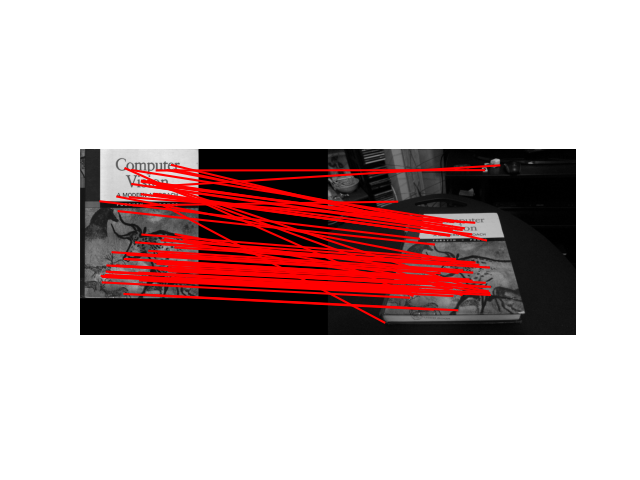
\includegraphics[width=\textwidth]{images/match-pics.png}
      \caption{Matched points}
      \label{fig:match-pics}
    \end{minipage}
  \end{figure}
\end{problem}

\newpage
\begin{problem}
  \textbf{BRIEF and Rotations}

  Let’s investigate how BRIEF works with rotations.
  Write a script \verb|briefRotTest.py| that:
  \begin{itemize}
    \item Takes the \verb|cvcover.jpg| and matches it to itself rotated
      [Hint: use \verb|scipy.ndimage.rotate|] in increments of 10 degrees.
    \item Stores a histogram of the count of matches for each orientation.
    \item Plots the histogram using \verb|matplotlib.pyplot.bar|
  \end{itemize}
  Include visualizations of the feature matching results at three
  different orientations. Explain why you think the BRIEF descriptor
  behaves this way.

  \begin{figure}[H]
    \centering
    \begin{minipage}{0.49\textwidth}
      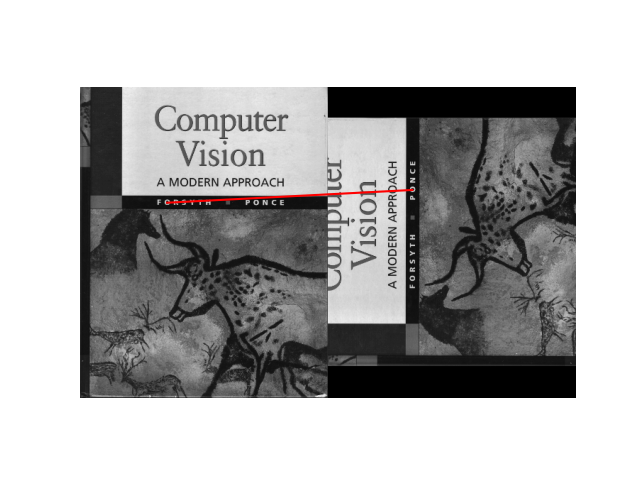
\includegraphics[width=\textwidth]{images/matches-90.png}
      \caption{rotation = $90$}
      \label{fig:threshold-0.03}
    \end{minipage}
    \begin{minipage}{0.49\textwidth}
      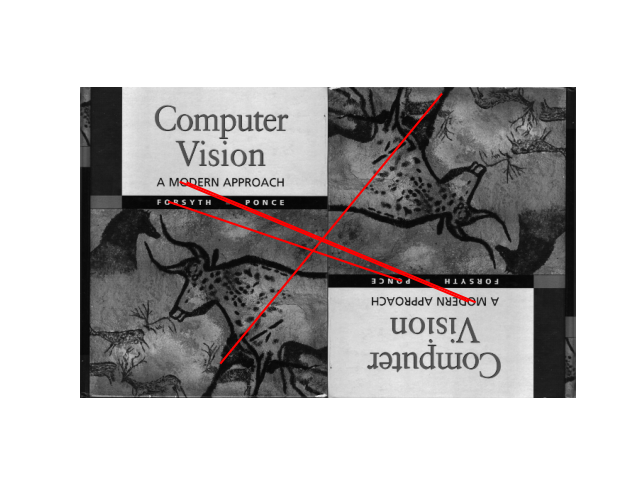
\includegraphics[width=\textwidth]{images/matches-180.png}
      \caption{rotation = $180$}
      \label{fig:threshold-0.3}
    \end{minipage}
    % \hfill
    \begin{minipage}{0.49\textwidth}
      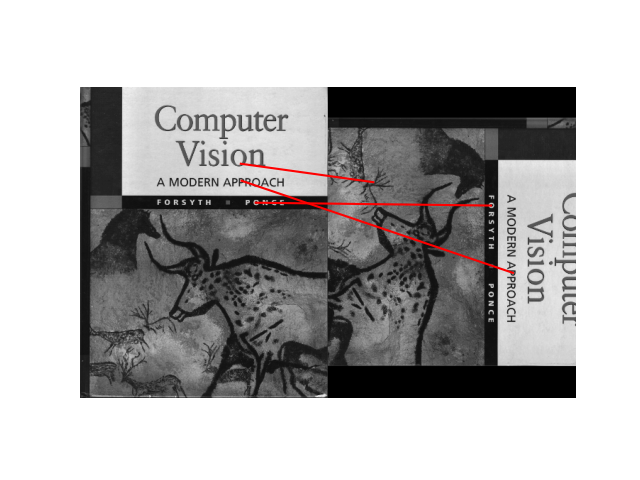
\includegraphics[width=\textwidth]{images/matches-270.png}
      \caption{rotation = $270$}
      \label{fig:matches-270}
    \end{minipage}
    \begin{minipage}{0.49\textwidth}
      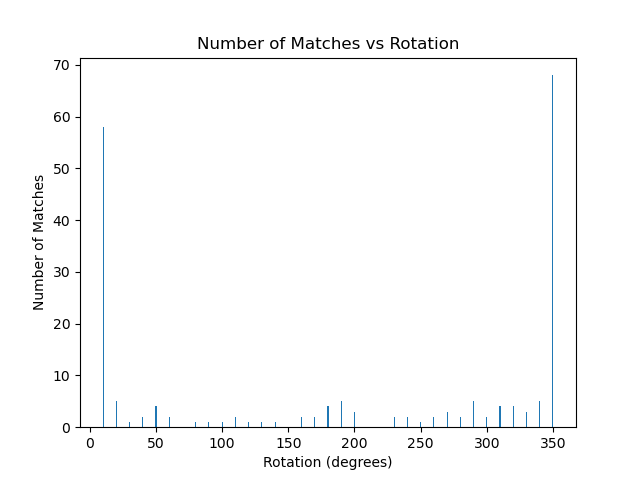
\includegraphics[width=\textwidth]{images/rotation_test.png}
      \caption{Match counts}
      \label{fig:match-counts}
    \end{minipage}
  \end{figure}
\end{problem}

We see the highest matches the more the two images are aligned
(rotations closer to $0$ or $360$ degrees).
This is to be expected, since the two images have a lot of similar
points when less rotated.

\newpage
\begin{problem}[9]
\textbf{Putting it Together} \\

\begin{figure}[H]
  \centering
  \begin{minipage}{0.51\textwidth}
    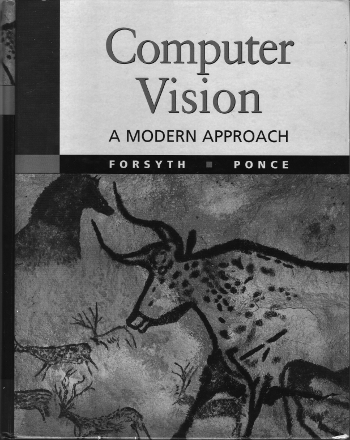
\includegraphics[width=\textwidth]{images/cv_cover.jpg}
    \caption{CV Book Cover}
    \label{fig:cv-cover}
  \end{minipage}
  % \begin{minipage}{0.49\textwidth}
  %   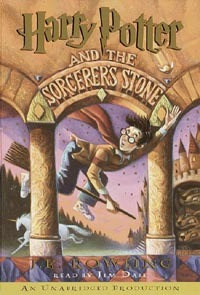
\includegraphics[width=0.1\textwidth]{images/hp_cover.jpg}
  %   \caption{Harry Potter Cover}
  %   \label{fig:hp-cover}
  % \end{minipage}
  \hfill
  \begin{minipage}{0.49\textwidth}
    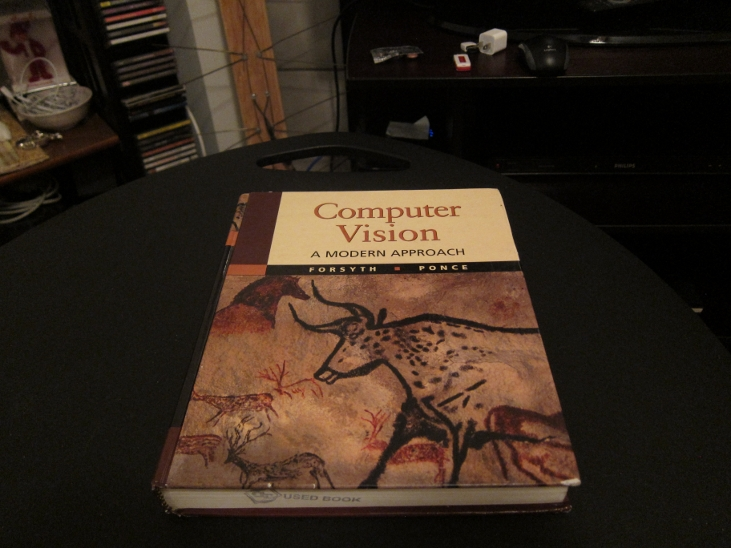
\includegraphics[width=\textwidth]{images/cv_desk.png}
    \caption{CV Book on Desk}
    \label{fig:cv-desk}
  \end{minipage}
  \begin{minipage}{0.49\textwidth}
    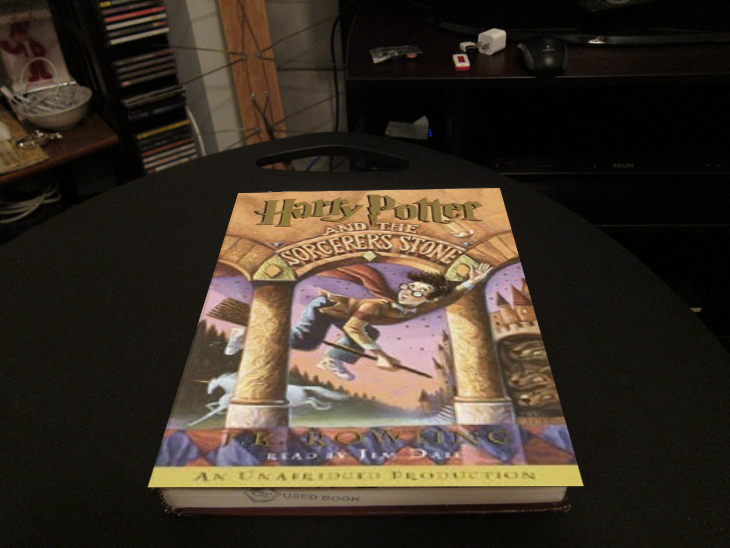
\includegraphics[width=\textwidth]{images/hp_desk.png}
    \caption{Harry Potter Book on Desk}
    \label{fig:hp-desk}
  \end{minipage}
\end{figure}

\begin{figure}[H]
  \centering
  \begin{minipage}{0.49\textwidth}
    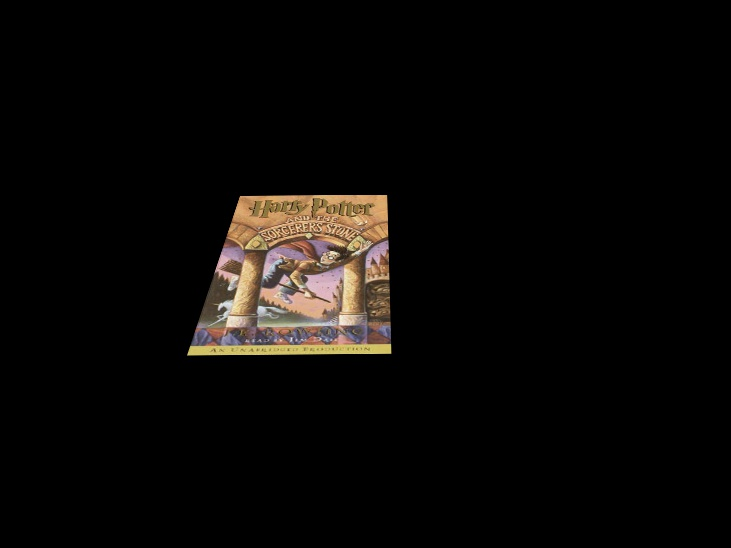
\includegraphics[width=\textwidth]{images/warped-cover.jpg}
    \caption{Warped Harry Potter Cover}
    \label{fig:warped-cover}
  \end{minipage}
  \begin{minipage}{0.49\textwidth}
    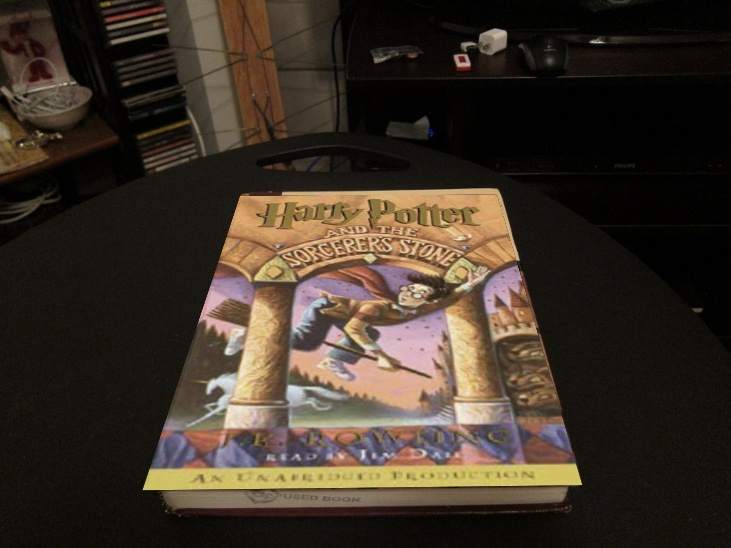
\includegraphics[width=\textwidth]{images/composite-image.jpg}
    \caption{Harry Potter-rized Image}
    \label{fig:composite-image}
  \end{minipage}
\end{figure}

\step
Because the original Harry Potter cover \verb|hp_cover.jpg| is smaller than
\verb|cv_cover.jpg|, it appears smaller when we warp it into the desk frame.
To make it appear the same size as the Computer Vision cover, we need to
rescale it to match the size of the Computer Vision cover.

\end{problem}

